\documentclass[a4paper, 11pt]{report}
\usepackage[margin=2cm]{geometry}
\usepackage{amsmath, amssymb, amsfonts, xcolor, mathtools, amsthm, float, booktabs, array}

\usepackage{tikz}
\usetikzlibrary{positioning}

\usepackage[ruled,vlined]{algorithm2e}
\usepackage{fancyhdr}
\usepackage{hyperref}
\usepackage[backend=biber,style=numeric,sorting=none]{biblatex}
\addbibresource{refs.bib}
\DefineBibliographyStrings{english}{bibliography={References}}

\DeclareMathOperator*{\argmax}{arg\,max}
\DeclareMathOperator*{\argmin}{arg\,min}
\newtheorem{definition}{Definition}
\newtheorem{proposition}{Proposition}
\newtheorem{theorem}{Theorem}
\theoremstyle{remark}
\newtheorem*{remark}{Remark}


\hypersetup{
    colorlinks=true,
    citecolor=teal,
    linkcolor=blue,
    urlcolor=magenta,
}
\newcommand{\R}{{\rm I\!R}}

\begin{document}
\chapter{Evolutionary Multiobjective Optimisation}
\section{Motivations}
    \begin{quote}
        \begin{itemize}
            \item Genetic Drift -- \href{https://en.wikipedia.org/wiki/Genetic_drift}{Wikipedia}
            \item Speciation -- \href{https://en.wikipedia.org/wiki/Speciation}{Wikipedia}
            \item Punctuated Equilbria -- \href{https://en.wikipedia.org/wiki/Punctuated_equilibrium}{Wikipedia}
        \end{itemize}
    \end{quote}
\section{Implications for Evolutionary Optimisation}
\paragraph{Implicit approaches}
    \begin{quote}
        Impose an equivalent of geographical separation. Impose an equivalent of speciation
    \end{quote}
\paragraph{Explicit approaches}
    \begin{quote}
        Make similar individuals compete for resources (fitness). Make similar individuals compete with each other for survival.
    \end{quote}
\subsection{Explicit 1: Fitness Sharing}
    \begin{quote}
        Restricts the number of individuals within a given niche by ``sharing'' their fitness, so as to allocate individuals to niches in proportion to the 
        niche fitness. Need to set the size of the niche $\sigma_{\text{share}}$. In either genotype or phenotype space run EA as normal but after each gen 
        set the shared fitness of each candidates with the equation of
        \begin{equation*}
            f'(i) = \frac{f(i)}{\displaystyle\sum_{j=1}^{\mu} sh\bigl(d(i,j)\bigr)}
            \qquad sh(d) =
            \begin{cases}
                1 - \dfrac{d}{\sigma}, & d < \sigma,\\[6pt]
                0, & \text{otherwise.}
            \end{cases} 
        \end{equation*}
    \end{quote}
\subsection{Explicit 2: Crowding}
    \begin{quotation}
        Attempts to distribute individuals \textbf{evenly} amongst niches. Relies on the assumption that offspring will tend to be close to parents.
        Uses a distance metric in phenotype/genotype space. Randomly shuffle and pair parents, then produce two offspring. Two parent/offspring tournaments - 
        pair so that 
        \[
            d(p_1, o_1) + d(p_2, o_2) < d(p_1, o_2) + d(p_2, o_1)
        \]
    \end{quotation}
\section{Prerequisites}
\subsection{Ordered Set}
\paragraph{Partial Ordered Set}
    \begin{quote}
        Formally, a partial order is a \textbf{homogeneous binary relation} that is \textbf{reflexive}, \textbf{antisymmetric}, and \textbf{transitive}. 
        A \textbf{partially ordered set} (\textit{poset} for short) is an \textit{ordered pair} $P = (X, \le)$ consisting of a set $X$ (called the 
        \textit{ground set} of $P$) and a partial order $\le$ on $X$. When the meaning is clear from context and there is no ambiguity about the partial 
        order, the set $X$ itself is sometimes called a poset.

        A \textbf{reflexive, weak,} or \textbf{non-strict partial order}, commonly referred to simply as a \textbf{partial order}, is a \textbf{homogeneous relation} $\le$ on a set $P$ that is \textbf{reflexive}, \textbf{antisymmetric}, and \textbf{transitive}. That is, for all $a, b, c \in P$, it must satisfy:
        \begin{enumerate}
            \item \textbf{Reflexivity:} $a \le a$, i.e. every element is related to itself.
            \item \textbf{Antisymmetry:} if $a \le b$ and $b \le a$ then $a = b$, i.e. no two distinct elements precede each other.
            \item \textbf{Transitivity:} if $a \le b$ and $b \le c$ then $a \le c$.
        \end{enumerate}
        A non-strict partial order is also known as an \textbf{antisymmetric preorder}.
    \end{quote}
\paragraph{Total Order}
    \begin{quote}
        In mathematics, a total order or linear order is a partial order \emph{\textbf{in which any two elements are comparable}}. That 
        is, a total order is a binary relation $\le$ on some set $X$, which satisfies the following for all $a, b$ and $c$ in $X$:
        \begin{enumerate}
            \item $a \le a$ (\textit{reflexive}).
            \item If $a \le b$ and $b \le c$ then $a \le c$ (\textit{transitive}).
            \item If $a \le b$ and $b \le a$ then $a = b$ (\textit{antisymmetric}).
            \item $a \le b$ or $b \le a$ (\textit{strongly connected}, formerly called \textit{totality}).
        \end{enumerate}
    \end{quote}
\subsection{Cartesian Product}
    \begin{quote}
        In \textbf{mathematics}, specifically \textbf{set theory}, the \textbf{Cartesian product} of two sets $A$ and $B$, denoted $A \times B$, is the set 
        of all \textbf{ordered pairs} $(a, b)$ where $a$ is an element of $A$ and $b$ is an element of $B$. In terms of \textbf{set-builder notation}, that is
        \[
            A \times B = \{(a, b) \mid a \in A \ \text{and} \ b \in B\}.
        \]
    \end{quote}
    \paragraph{Orders on the Cartesian product of totally ordered sets}
        \begin{quote}
            There are several ways to take two totally ordered sets and extend to an order on the \textbf{Cartesian product}, though the resulting order may 
            only be \textbf{partial}. Here are three of these possible orders, listed such that each order is stronger than the next:
            \begin{itemize}
                \item \textbf{Lexicographical order:} $(a,b) \le (c,d)$ if and only if $a < c$ or $(a = c \text{ and } b \le d)$. This is a total order.
                \item $(a,b) \le (c,d)$ if and only if $a \le c$ and $b \le d$ (the \textbf{product order}). This is a partial order.
                \item $(a,b) \le (c,d)$ if and only if $(a < c \text{ and } b < d)$ or $(a = c \text{ and } b = d)$ (the reflexive closure of the \textbf{direct product} of the corresponding strict total orders). This is also a partial order.
            \end{itemize}
        \end{quote}
    \paragraph{Relations as Subsets of Cartesian Products}\href{https://math.stackexchange.com/questions/2454926/relations-cartesian-product-explanation}{Mathematics Exchange}
        \begin{quote}
            The set of ordered pairs drawn from the Cartesian product can be defined as
            \begin{equation*}
                R = \left\{(x,y)\in A\times B|\;xRy\right\}
            \end{equation*}
            Thus we can say
            \begin{equation*}
                R\subseteq A\times B
            \end{equation*}
        \end{quote}
\section{Multiobjective Optimisation}
    \begin{quote}
        Many problems have more than one goal function thus there is no single optimal function value. There is a general assumption that MO is as hard as Single-objective optimisation. We have 
        the decision space of $S^n$ with $s\in S^n$ and with our objective function $\mathsf{F}(f_1(s),f_2(s),\ldots,f_m(s))$ will yield the objective space of $\R^m$. Therefore, for a general 
        MOP we have that 
        \begin{equation*}
            \mathsf{F}: S^n\to\R^m,\quad\text{where } n<m\vee n>m\vee n=m
        \end{equation*}
        We say $x\in\R^m$ dominates $y\in\R^m$ if it is at least as good on all criteria and better on at least one.
    \end{quote}
    \paragraph{Dominance in the Objective Space}
        \begin{quote}
            Assuming maximisation
            \begin{quote}
                $x$\emph{ weakly dominates }$y$ ($x\succeq y$) iff $x_i\geq y_i\;\forall\,i\in\{1,\ldots,m\}$\\
                $x$\emph{ dominates }$y$ ($x\succ y$) iff $x\succeq y$ and $x\neq y$
            \end{quote}
            This can be translated to the search space as
            \begin{equation*}
                \begin{aligned}
                    s\succeq s^\prime\iff\mathsf{F}(s)\succeq\mathsf{F}(s^\prime)\\
                    s\succ s^\prime\iff\mathsf{F}(s)\succ\mathsf{F}(s^\prime)
                \end{aligned}
            \end{equation*}
        \end{quote}
    \paragraph{Pareto Front -- \href{https://en.wikipedia.org/wiki/Pareto_front}{Wikipedia}}
        \begin{quote}
            The Pareto Front consists of all the non-dominated objective vectors. Let $\boldsymbol{\pi}\subseteq\R^m$ be the set of feasible objective vectors
            such that
            \begin{equation*}
                \boldsymbol{\pi} = \{\pi\in\R^m: \pi = \mathsf{F}(s)\text{ where }s\in S^n\}
            \end{equation*}
            For any objective vectors $\pi^\prime,\pi^{\prime\prime}\in\boldsymbol{\pi}$, let $\mathsf{P}(\boldsymbol{\pi})$ be the Pareto set thus
            \begin{equation*}
                \mathsf{P}(\boldsymbol{\pi}) = \bigl\{\pi^\prime: \{\pi^{\prime\prime}\succ\pi^\prime\} = \emptyset\bigr\}
            \end{equation*}
        \end{quote}
    \paragraph{Parento Optimal}
        \begin{quote}
            A solution $x^*\in X$ is then called \emph{Parento Optimal} iff there is no other solution in $X$ that dominates $x^*$ \fbox{\cite{brockhoff2009theoretical}}.
        \end{quote}
    \paragraph{Pareto set approximations}
        \begin{quote}
            Specific sets of solutions are the so-called \emph{Pareto set approximations}, which are solution sets of pairwisely non-dominated solutions \fbox{\cite{brockhoff2009theoretical}}.
        \end{quote}
    \paragraph{EC for Parento Front}
        \begin{quote}
            Population-based nature of search means you can simultaneously search for set of points approximating Pareto front. Don't have to make guesses about which combinations of weights
            might be useful. Don't have to make guesses about which combinations of weights might be useful.
        \end{quote}
\subsection{NSGA-II}
    \begin{quote}
        The non-dominated sorting GA-II is an elitist approach which rank and preserve the best solution on top. In order to sort a population of $N$ size
        each solution must be compared with every other solution in the population to find if it is dominated. This requires $\mathcal{O}(MN)$ where $M$ 
        is the number of objective vectors. When this process is continued to find the members of the first non-dominated class for all population members
        the total complexity is $\mathcal{O}(MN^2)$. At this stage, all individuals in the first non-dominated front are found. In order to find the next front
        repeat the above procedure. As can be seen the worst case (when there exists only one solution in each front) complexity of this algorithm is 
        $\mathcal{O}(MN^3)$. The fast NSGA-II will require at most $\mathcal{O}(MN^2)$ computations. In the following algorithm, it's worth mentioning 
        that the space complexity is $\mathcal{O}(N^2)$. \fbox{\cite{deb2000nsga2}}. Please refer to the pseudo-code in the \emph{lecture slide}.
    \end{quote}
\subsection{Crowding Distance}
    \begin{quote}
        To get an estimate of the density of solutions surrounding a particular point in the population we take the average distance of the two points on 
        either side of this point along each of the objective vectors. This quantity $i_{\text{distance}}$ serves as an estimate of the size of the largest cuboid 
        enclosing the point $i$ without including any other point in the population. The time complexity for the sorting is $\mathcal{O}(MN\log N)$ \fbox{\cite{deb2000nsga2}}. 
        Please refer to the \emph{lecture slide} for the pseudo-code and illustration. 
    \end{quote}
\subsection{Crowding Comparison Operator}
    \begin{quote}
        The crowded comparison operator ($\succ_n$) guides the selection process at the various stages of the algorithm towards a uniformly spread out Pareto-optimal front. This helps
        to have a more diverse solution set \fbox{\cite{deb2000nsga2}}.
        \begin{enumerate}
            \item Non-domination rank -- $i_{rank}$
            \item Local crowding distance -- $i_{distance}$
        \end{enumerate}
        \begin{equation*}
            i \succ_n j \;\text{ if }\;
            (i_{rank} < j_{rank}) \;\text{or}\;
            \big( (i_{rank} = j_{rank}) \;\text{and}\; (i_{distance} > j_{distance}) \big)
        \end{equation*}
    \end{quote}
\subsection{Iteration for NSGA-II}
    \begin{center}
        Please refer to the \emph{lecture slide} for the pseduo-code. 
    \end{center}
    \begin{quote}
        Initially, a random parent population ?p is created. The population is sorted based on the non-domination. Each solution is assigned a fitness equal to its non-domination level 
        (1 is the best level). Thus, minimization of fitness is assumed. Binary tournament selection, recombination, and mutation operators are used to create a child population $Q_0$ of size
        $N$. Let us now look at the complexity of one iteration of the entire algorithm. The basic operations being performed and the worst-case complexities associated with them are as follows:
        \begin{enumerate}
            \item Non-dominated sort is $O(MN^2)$,
            \item Crowding distance assignment is $O(MN \log N)$, and
            \item Sort on $\ge_n$ is $O(2N \log(2N))$.
        \end{enumerate}
        As can be seen, the overall complexity of the above algorithm is $\mathcal{O}(MN^2)$ \fbox{\cite{deb2000nsga2}}.
    \end{quote}
\subsection{Deteriorative Cycles}  
    \begin{quote}
        In single-objective optimization, every solution is mapped to a real value and solutions can always be pairwisely compared via the less or equal 
        relation $\leq$ on $\R$. In another words, the total order (any elements are comparable) $\leq\subseteq\R\times\R$ induces via $f$ order on the 
        search space $X$ that is a total preorder. In a multiobjective scenario, the $\le$ relation is generalized to objective vectors, i.e., $\le$ is 
        a subset of $\R^k\times\R^k$. Here, the totality is not given due to vectors $a, b \in \R^k$ where $f_1(a) < f_1(b)$ 
        but $f_2(a) > f_2(b)$—the relation $\le$ on the set of objective vectors is only a partial order, i.e., reflexive, antisymmetric, and transitive. 
        This means that \emph{not any elements are comparable}. \fbox{\cite{brockhoff2009theoretical}}
    \end{quote}
\subsubsection{Downfall of The Evolutionary Algorithm Multiobjective Optimisation}
    \begin{quote}
        Among the well-established ones, NSGA-II [Deb et al., 2002] and SPEA2 [Zitzler et al., 2002] have to be mentioned here. Both use the Pareto dominance 
        concept as the main selection criterion in an elitist manner where non-dominated solutions are favored over dominated ones. In addition, a second selection 
        criterion establishes diversity among the solutions. However, experimental studies have shown that both algorithms do not scale well if the number 
        of objectives increases and that a cyclic behavior can be observed. This means that—although non-dominated solutions are preferred over dominated 
        ones—over time, previously dominated solutions enter the population again, resulting in an oscillating distance to the Pareto front.
        \fbox{\cite{brockhoff2009theoretical}}
    \end{quote}
\subsection{Hypervolume Indicator}
    \begin{quote}
        One of the latest areas of evolutionary multiobjective optimization where theoretical investigations have been made is the area of hypervolume-based search. The hypervolume indicator, 
        initially proposed for performance assessment, has nowadays been used to guide the search in several multiobjective evolutionary algorithms such as the SMS-EMOA of Beume et al. [2007b], 
        the multiobjective version of CMA-ES [Igel et al., 2007], or HypE [Bader and Zitzler, 2008, 2009]. As mentioned above, the hypervolume indicator is a unary quality measure mapping a set 
        of solutions to the hypervolume in objective space that is dominated by the corresponding objective vectors of the solutions but not by a predefined set of \emph{reference points}. 
        More formally, for a given set $A\subseteq S^n$ of a solution set and set of reference points in the objective space $R\subseteq\R^m$. We define the set of objective vectors that are 
        dominated by $A$ but not by $R$ as \fbox{\cite{brockhoff2009theoretical}}
        \begin{equation*}
            H(A,R) = \{h: \exists\,a\in A,\;\exists\,r\in R: \mathsf{F}(a)\leq h\leq r\}
        \end{equation*}
        And the corresponding hypervolume indicator with reference $R$ is $I^{R}_{H}$ as
        \begin{equation*}
            I^R_H\coloneq\text{VOL}\left(\bigcup_{s\in A}\big[f_1(s),r_1\big]\times\big[f_2(s),r_2\big]\times\ldots\times\big[f_m(s),r_m\big]\right),\quad\text{ where } 
            \begin{cases}
                r_i\in R\subseteq\R^m\\
                s\in A
            \end{cases}
        \end{equation*}
        This means the objective value with the corresponding reference point.
    \end{quote}
\chapter{Submodular function}
    \begin{minipage}{0.45\linewidth}
        \begin{algorithm}[H]
            \caption{Generalized Cost-benefit Algorithm}
            \KwData{$B > 0$}
            \KwResult{Selection $S \subseteq V$}
            $v^* := \arg\max \{ f(v) \mid v \in V, \hat{c}(v) \leq B \}$\;
            $G := \emptyset$\;
            $V' := V$\;

            \While{$V' \neq \emptyset$}{
                \ForEach{$X \in V$}{
                    $\Delta^X_f := f(G \cup X) - f(G)$\;
                    $\Delta^X_c := \hat{c}(G \cup X) - \hat{c}(G)$\;
                }
                $X^* = \arg\max \left\{ \Delta^X_f/\Delta^X_c \mid X \in V' \right\}$\;
                
                \If{$\hat{c}(G \cup X^*) \leq B$}{
                    $G := G \cup X^*$\;
                }
                $V' := V' \setminus X^*$\;
            }
            \Return{$\arg\max_{S \in \{v^*, G\}} f(S)$}\;
        \end{algorithm}
    \end{minipage}
    \begin{minipage}{0.45\linewidth}
        \begin{algorithm}[H]
            \caption{Generalized Greedy Algorithm}
            \KwIn{Initial budget constraint $B$}
            \KwOut{Selection $S \subseteq V$}

            $X \leftarrow \emptyset$\;
            $V' \leftarrow V$\;

            \Repeat{$V' = \emptyset$}{
                $v^* \leftarrow \arg\max_{v \in V'} \frac{f(X \cup v) - f(X)}{\hat{c}(X \cup v) - \hat{c}(X)}$\;
                
                \If{$\hat{c}(X \cup v^*) \le B$}{
                    $X \leftarrow X \cup v^*$\;
                }
                $V' \leftarrow V' \setminus \{v^*\}$\;
            }

            $v^* \leftarrow \arg\max_{v \in V, \, \hat{c}(v) \le B} f(v)$\;
            \Return{$\arg\max_{S \in \{X, \{v^*\}\}} f(S)$}\;
            \vspace{4.2em}
        \end{algorithm} 
    \end{minipage}\\[1em]
    \noindent
    \framebox[\textwidth][l]{
        \parbox{0.97\textwidth}{
            \textbf{Approximate Local Search Procedure B:}

            \medskip
            \textbf{Input:} Ground set \( X \) of elements and value oracle access to submodular function \( f \).

            \begin{enumerate}
                \item Let \(\{v\}\) be a singleton set with the maximum value \( f(\{v\}) \) and let \( S = \{v\} \).
                \item While there exists the following delete or exchange local operation that increases the value of \( f(S) \) by a factor of at least \( 1 + \frac{\epsilon}{n^4} \), then apply the local operation and update \( S \) accordingly.
                \begin{itemize}
                    \item \textbf{Delete operation on \(S\).} If \( e \in S \) such that \( f(S \setminus \{e\}) \ge (1 + \frac{\epsilon}{n^4}) f(S) \), then \( S \leftarrow S \setminus \{e\} \).
                    \item \textbf{Exchange operation on \(S\).} If \( d \in X \setminus S \) and \( e_i \in S \cup \{\phi\} \) (for \( 1 \le i \le k \)) are such that \((S \setminus \{e_1, \ldots, e_k\}) \cup \{d\} \in \mathcal{I}_i\) for all \( i \in [k] \) and \( f((S \setminus \{e_1, \ldots, e_k\}) \cup \{d\}) > (1 + \frac{\epsilon}{n^4}) f(S) \), then \( S \leftarrow (S \setminus \{e_1, \ldots, e_k\}) \cup \{d\} \).
                \end{itemize}
            \end{enumerate}
        }
    }
\section{Global-SEMO}
    \begin{quote}
        The use of one-bit mutations is attractive for theoretical investigations as its analysis is often easier compared to other mutation operators. It
        is, however, only a \emph{local search operator} flipping one bit at a time and therefore does not guarantee a finite running time for all pseudo-Boolean
        functions. On the contrary, the independent-bit mutation operator, which flips each bit independently with a certain probability, can be called a 
        \emph{global search} operator since it can produce any point in the decision space with positive probability.\\
        \cite{laumanns2004running}.
    \end{quote}
    \begin{algorithm}[H]
        \caption{GSEMO (concise)}
        \KwIn{Objective $g:\{0,1\}^n \to \mathbb{R}^m$}
        \KwOut{Pareto set $P$}
        $x \sim \mathrm{Unif}(\{0,1\}^n)$\;
        $P \gets \{x\}$\;
        \Repeat{stop}{
            pick $x \in P$ u.a.r.\tcp*{uniformly at random}
            $x' \gets \mathrm{flip}_{1/n}(x_i)\;\forall\,i$ \tcp*{flip each bit independently w.p.\ $1/n$}
            compute $g(x')$\;
            \If{$\nexists\, y\in P:\; g(y)\prec g(x')$}{
                $P \gets (P \cup \{x'\}) \setminus \{y\in P:\; g(y)\preceq g(x')\}$\;
            }
        }
        \Return{$P$}
    \end{algorithm}
\subsection{Knapsack Problem on GSEMO \cite{laumanns2004running}}
\begin{quote}
The optimization problem considered in this study is a special instance of the multiobjective knapsack problem. Given is a set of $n$ items, each 
of which has $m$ profit and $k$ weight values associated with it. The goal is to select a subset of items such that the sums over each of their 
$k$-th weight values do not exceed given bounds and the sums over each of their $m$-th profit values are maximized.
\end{quote}
\begin{definition}[Pareto optimality]
Let $f : X \to F$, where $f$ is called the \textit{objective function}, $X$ the \textit{decision space}, and 
$F \subseteq \mathbb{R}^m$ the \textit{objective space}. The elements of $X$ are called \textit{decision vectors} 
and the elements of $F$ \textit{objective vectors}. 

Let $X' \subseteq X$ denote the set of feasible decision vectors, i.e., decision vectors fulfilling the constraints. 
A feasible decision vector $x^* \in X'$ is \textit{Pareto optimal} if there is no other $x \in X'$ that dominates 
$x^*$. The vector $x$ dominates $x^*$, denoted as $x \succ_f x^*$, if $f_i(x) \ge f_i(x^*)$ for all $i = 1, \ldots, m$ 
and $f_i(x) > f_i(x^*)$ for at least one index $i$.

The set of all Pareto optimal decision vectors $X^*$ is called the \textit{Pareto set}. 
The corresponding set $F^* = f(X^*)$ is the set of all Pareto optimal objective vectors and is 
denoted as the \textit{Pareto front}.
\end{definition}

\begin{definition}[MOKP]
Let $X=\{0,1\}^n$ be the decision space and $n\in\mathbb{N}$. The Multiobjective Knapsack Problem (MOKP) is
\begin{equation*}
    \argmax_{x\in X}f(x)=\bigl(f_1(x),f_2(x)\bigr)
    \qquad
    \mathrm{s.t}\quad g(x)\le \tfrac{n}{2},
\end{equation*}
with
\[
f_1(x)=\sum_{i=1}^{n}2^{\,n-i}x_i,\qquad
f_2(x)=\sum_{i=1}^{n}2^{\,i-1}x_i,\qquad
g(x)=\sum_{i=1}^{n}x_i,\qquad
x=(x_1,\ldots,x_n)\in X^n.
\]
\end{definition}

\paragraph{Pareto set size and structure.}
The MOKP function is a bijection, so none of the $|X|=\Theta(2^n)$ decision vectors maps to the same objective vector. 
The Pareto set contains $|X^*|=n^2/4+1$ elements and has the form below.

\begin{proposition}\label{prop:type-forms}
A decision vector $x\in X$ is Pareto-optimal in the MOKP problem if and only if it has the form
\[
\underbrace{(1,1,\ldots,1}_{a},
\underbrace{0,0,\ldots,0}_{n/2},
\underbrace{1,1,\ldots,1)}_{n/2-a}
\qquad\text{(Type 1)}
\]
or
\[
\Bigl(
\underbrace{1,1,\ldots,1}_{b},
\underbrace{0,0,\ldots,0}_{c},
1,
\underbrace{0,0,\ldots,0}_{\tfrac{n}{2}-c},
\underbrace{1,1,\ldots,1}_{\tfrac{n}{2}-b-1}
\Bigr),\qquad\text{(Type 2)}
\]
where $a\in\{0,1,\ldots,n/2\}$, $b\in\{0,1,\ldots,n/2-1\}$, and $c\in\{1,\ldots,n/2-1\}$.
\end{proposition}

\begin{proof}[Informal proof sketch]
Firstly only the decision vector with size $\leq 1/2$ can be inside the Pareto-optimal set. Thus there exists a vector with 
$p,q\in\{2,3,\ldots,n\}$ where $p>q$ such that $x_p=x_q=1$ and $x_{p-1}=x_{q+1}=0$. By inverting those bits, for the first objective function we have the gain 
$2^{n-p}-2^{n-q-1}>0$, and for the second objective function we have the gain $2^{q-1}-2^{p-2}>0$. As the first objective favors small indices and the second 
favors large indices, maximizing one requires compensating in the other; hence the one-bit is pushed toward both sides.
\end{proof}

\paragraph{Supported solutions.}
Only the $n/2+1$ Pareto-optimal decision vectors of the first type are `supported' solutions. A solution is supported if there exists a weight 
combination such that it maximizes the weighted sum $\sum_{i=1}^{m}w_i f_i(x)$ (a single-objective surrogate).

\begin{proposition}\label{prop:supported}
Let $\Phi(x)\overset{\text{def}}{=}w f_1(x)+(1-w)f_2(x)$, where $w\in[0,1]$. 
For each Pareto-optimal decision vector $x''$ of Type~2 and each $w\in[0,1]$, there exists some Pareto-optimal vector $x'$ of Type~1 such that 
$\Phi(x')>\Phi(x'')$.
\end{proposition}

\begin{proof}
Let w.l.o.g.\ $x''$ be a Pareto-optimal vector of Type~2, where the bit with index $b+c+1$ is set to one. Let $x',x'''$ be defined as the two vectors 
identical with $x''$ at $n-2$ positions, where only this one-bit is moved to position $b+1$ and $n/2+b+1$, respectively. Clearly, these $x',x'''$ belong to 
Type~1. We show that $(\Phi(x')+\Phi(x'''))/2>\Phi(x'')$, which implies that at least one of $\Phi(x')$ and $\Phi(x''')$ is larger than $\Phi(x'')$:
\[
(\Phi(x')+\Phi(x'''))/2>\Phi(x'')
\]
\[
\Leftrightarrow\;
w\!\left(2^{\,n-b-2}+2^{\,n-n/2-b-2}\right)
+(1-w)\!\left(2^{\,b-1}+2^{\,n/2+b-1}\right)
>
w\,2^{\,n-b-c-1}+(1-w)\,2^{\,b+c}
\]
\[
\Leftrightarrow\;
w\!\left(2^{-1}+2^{-n/2-1}\right)
+(1-w)\!\left(2^{-1}+2^{\,n/2-1}\right)
>
w\,2^{-c}+(1-w)\,2^{\,c}.
\]
The last inequality holds for $1\le c\le n/2-1$, which covers all possible Type~2 vectors by Proposition~\ref{prop:type-forms}. \qedhere
\end{proof}
\begin{remark}[On the choice of $x'$ and $x'''$]
    I am considering why the author uses the first 0 bit in the middle section for Type~1 (in \(x'\)) and the last 0 bit before the right section of 1s (in \(x'''\)). 
    I am guessing that this is because these positions produce the smallest possible maximization for one objective while minimizing the gain in the other. 
    On the left block of 1s, the outermost position yields the least value for \(f_1\) (due to exponential decay), so moving the isolated 1 to the start of the middle 0s 
    (for \(x'\)) provides only a modest boost to \(f_1\) but significantly reduces \(f_2\). Similarly, for \(x'''\), moving it to the end of the middle 0s (just before the 
    right 1s) modestly boosts \(f_2\) but greatly penalizes \(f_1\). The logic is symmetric for the second objective. These are the ``minimal improvement'' moves closest to \(x''\); 
    if \((\Phi(x')+\Phi(x'''))/2>\Phi(x'')\) already holds here, it holds for any farther move (which improves even more), confirming that no Type~2 vector can be supported.
\end{remark}
\begin{quote}
Our goal is therefore to investigate how long different multiobjective EAs take to find the whole Pareto set $X^*$ of MOKP. 
The algorithms we consider are the SEMO (Simple Evolutionary Multiobjective Optimizer) and the FEMO 
(Fair Evolutionary Multiobjective Optimizer). In contrast to the original version of Laumanns et al.\ (2002), 
we use the independent-bit mutation, which results, according to the definition of Giel (2003), 
in the global SEMO and global FEMO. 

Both algorithms were so far only applied to unconstrained problems, so the question arises of how to deal 
with the constraint here. Our idea is to adapt and generalize the order relation of Definition~1, 
which so far only involves the objectives and ignores the constraints. 
This approach makes it unnecessary to incorporate a dedicated constraint-handling technique 
in the definition of the algorithm. The algorithms can therefore remain unchanged.
\end{quote}

\section{Basics of Matroid Theory \cite{hillman_matroid_2016}}
    \begin{quote}
        A matroid is a structure that generalizes the \emph{properties of independence}. Relevant applications are found in graph theory and linear algebra. There are several ways to define a matroid, 
        each relate to the concept of independence. This paper will focus on the the definitions of a matroid in terms of bases, the rank function, independent sets and cycles.
        To understand the matroid being used in the evolutionary algorithm it is best to understand it as the intuition of a graph. The notation for 
        matroid can be written as 
        \begin{equation*}
            \mathcal{M} = (E,\mathcal{I})\qquad\text{or}\qquad\mathcal{M} = (E,B)
        \end{equation*}
        Those notation can be defined below.
    \end{quote}
\subsection{Bases}
    \begin{definition}
        A matroid $\mathcal{M}$ consists of a non-empty finite set $E$ and a non-empty collection $B\subseteq 2^E$, called bases, satisfying the following properties:
        \begin{itemize}
            \item[i] No base properly contains another base
            \item[ii] If $B_1$ and $B_2$ are bases and if any $e\in B_1$, then there is a $f\in B_2$ such that $(B_1\setminus e)\cup f$ is also a base.
        \end{itemize}
    \end{definition}
    \begin{theorem}
        Every base of a matroid has the same number of elements  
    \end{theorem}
    \begin{remark}[On Theorem 1]
        The above theorem can be easy proof by the base of the linear space. We can take it for granted.
    \end{remark}
    \begin{figure}[H]
        \centering
        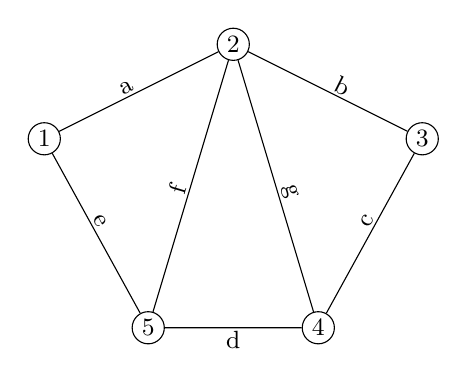
\begin{tikzpicture}[scale=1.2,
        vertex/.style={circle,fill=white,draw=black,inner sep=1.5pt,font=\small},
        elabel/.style={midway,sloped,fill=none,inner sep=1pt,font=\small}
    ]
    %--- vertices ---
    \node[vertex] (v2) at (0,2) {2};
    \node[vertex] (v1) at (-2,1) {1};
    \node[vertex] (v3) at ( 2,1) {3};
    \node[vertex] (v5) at (-0.9,-1) {5};
    \node[vertex] (v4) at ( 0.9,-1) {4};

    %--- edges ---
    \draw (v1)-- node[elabel,above left] {a} (v2);
    \draw (v2)-- node[elabel,above right]{b} (v3);
    \draw (v3)-- node[elabel,above right]      {c} (v4);
    \draw (v5)-- node[elabel,below]      {d} (v4);
    \draw (v1)-- node[elabel,above left]       {e} (v5);
    \draw (v2)-- node[elabel,above left]       {f} (v5);
    \draw (v2)-- node[elabel,above right]      {g} (v4);
\end{tikzpicture}
        \caption{Graph $G$}
    \end{figure}
    \begin{quote}
        We will take a base of our matroid to be a \emph{spanning tree} of $G$.
    \end{quote}
    \begin{table}[h]
        \centering
        \begin{tabular}{c}
            \multicolumn{1}{c}{\Large\textbf{Bases}}\\
            \cmidrule(lr){1-1}
            $\{a,b,c,d\}$\\
            $\{a,e,d,c\}$\\
            $\{b,c,d,e\}$\\
            $\{b,a,e,d\}$\\
            $\{c,b,a,e\}$\\
            $\{c,b,f,e\}$\\
            $\{c,d,f,a\}$\\
            $\{c,g,a,e\}$\\
            $\{c,g,f,e\}$\\
        \end{tabular}
        \caption{The Spanning Trees of $G$}
        \label{tab:spanning-trees-G}
    \end{table}
\subsection{Rank function}
    \begin{definition}
        A matroid consists of a non-empty finite set E and an integer-valued function r defined on the set of subset of E, satisfying:        
        \begin{itemize}
            \item[i] $0\leq r(A)\leq |A|$, for each $A\subseteq E$ 
            \item[ii] If $A\subseteq B\subseteq E$, then $r(A) \leq r(B)$
            \item[iii] For any $A,B\subseteq E$, $r(A\cup B) + r(A\cap B)\leq r(A) + r(B)$
        \end{itemize}
    \end{definition}
    \begin{theorem}
        The rank of M equals the size of a base of M.
    \end{theorem}
\subsection{Independent Set}
    \begin{definition}
        A matroid $\mathcal{M}$ consists of a non-empty finite set E and a non-empty collection $\mathcal{I}\subseteq 2^E$ (called independence set) 
        satisfying the following properties:
        \begin{itemize}
            \item[i] Any subset of an independent set is independent
            \item[ii] If I and J are independent sets with $|J|>|I|$ then there is an element e such that $e\in J \wedge e\notin I$. Thus $I\cup e$ is 
            independent.
        \end{itemize}
    \end{definition}
    \begin{definition}
        We will take the independent sets of a graph to be the sets of edges in a graph that do not contain a cycle. A forest is a graph that contains 
        no cycles. A connected forest is a tree.
    \end{definition}
    \begin{table}[H]
        \centering
        \renewcommand{\arraystretch}{1.2}
        \begin{tabular}{>{\centering\arraybackslash}m{0.8\linewidth}}
            \multicolumn{1}{c}{\Large\textbf{Forests of $G$}}\\
            \cmidrule(lr){1-1}
            $\{a\}, \{b\}, \{c\}, \{d\}, \{e\}$\\
            $\{f\}, \{g\}, \{a,b\}, \{b,c\}$\\
            $\{c,d\}, \{d,e\}, \{e,f\}, \{f,g\}$\\
            $\{g,a\}, \{a,f\}, \{e,f\}, \{d,f\}$\\
            $\{b,f\}, \{b,g\}, \{c,g\}, \{d,g\}$\\
            $\{a,b,c\}, \{a,b,g\}, \{a,e,d\}$\\
            $\{a,f,d\}, \{a,g,c\}, \{a,g,d\}$\\
            $\{b,c,d\}, \{b,g,d\}, \{b,f,d\}$\\
            $\{b,f,e\}, \{c,d,e\}, \{c,g,d\}$\\
            $\{c,d,f\}, \{e,f,e\}, \{a,f,g\}$\\
            $\{a,b,c,d\}, \{a,e,d,c\}, \{b,c,d,e\}$\\
            $\{b,a,e,d\}, \{c,b,a,e\}, \{c,b,f,e\}$\\
            $\{c,d,f,a\}, \{c,g,a,e\}, \{c,g,f,e\}$\\
        \end{tabular}
        \caption{The Forests of $G$}
        \label{tab:forests-G}
    \end{table}

\newpage
\printbibliography
\end{document}